\chapter{Results and Discussion}
\label{sec:chapterResults}

% ══════════════════════════════════════════════════════════════════════════
% REQUIRED PACKAGES (add to main .tex preamble if not already present):
%   \usepackage{pgfplots}
%   \pgfplotsset{compat=1.18}
%   \usepgfplotslibrary{groupplots}
%   \usepackage{booktabs}
%   \usepackage{xcolor}       % for \definecolor
%   \usepackage{multirow}     % for multi-row cells (optional)
% ══════════════════════════════════════════════════════════════════════════

% NOTE: All numeric values are illustrative placeholders (dummy).
% They will be replaced with actual experimental results as each code step completes.
% The structure, metrics, and table layout are final and aligned with the Methodology chapter.

% ── Consistent model colours for all figures ──
\definecolor{clrLGBM}{HTML}{1f77b4}
\definecolor{clrCB}{HTML}{d62728}
\definecolor{clrRF}{HTML}{2ca02c}
\definecolor{clrFT}{HTML}{ff7f0e}
\definecolor{clrLR}{HTML}{9467bd}
\definecolor{clrOCSVM}{HTML}{7f7f7f}

\section{Results}
\label{sec:results}

This section is organised in practical execution order:
each subsection corresponds to a well-defined experimental step whose artefacts (tables, figures, metrics JSON files) are produced by a specific code pipeline run.
Sections are numbered sequentially—no phase labels are used.
All metrics are defined in Section~\ref{sec:metrics} of the Methodology chapter.

% ══════════════════════════════════════════════════════════════════════════
%  1 — BASELINE MODEL COMPARISON
% ══════════════════════════════════════════════════════════════════════════
% CODE STEP 1:
%   python main.py --dataset ulb    --models all --strategy none
%   python main.py --dataset baf_base --models all --strategy none
% Produces: metrics_test.json, pr_curve_data.json, confusion_matrix.png
%           for each model on each dataset.
% ══════════════════════════════════════════════════════════════════════════

\subsection{Baseline Model Comparison (No Imbalance Strategy)}
\label{sec:baseline_results}

This section compares all models tuned via 5-fold stratified cross-validation
(scoring\,=\,PR-AUC) \emph{without} any imbalance handling strategy.
Results are reported on the holdout test set using the
$F_2$-maximising threshold~($\tau$) obtained from inner validation
(median across folds).
The same trained models and probability scores are later reused for
the threshold sensitivity analysis (Section~\ref{sec:threshold_sensitivity}),
where alternative threshold strategies are applied \emph{without retraining}.

% ─────────────────── ULB 2013 ───────────────────

\subsubsection{ULB Credit Card 2013}

\begin{table}[ht]
\centering
\caption{Baseline comparison on ULB 2013 (strategy\,=\,None, threshold\,=\,max-$F_2$).}
\label{tab:baseline_ulb}
\begin{tabular}{l c c c c c c c}
\toprule
Model & PR-AUC & $F_1$ & $F_2$ & Precision & Recall & $\tau$ & Brier \\
\midrule
LR        & 0.742 & 0.758 & 0.809 & 0.569 & 0.878 & 0.176 & 0.0012 \\
RF        & 0.838 & 0.842 & 0.831 & 0.878 & 0.816 & 0.342 & 0.0009 \\
LGBM      & 0.865 & 0.863 & 0.847 & 0.912 & 0.827 & 0.285 & 0.0008 \\
CatBoost  & 0.858 & 0.855 & 0.840 & 0.901 & 0.820 & 0.298 & 0.0008 \\
FT-Trans. & 0.851 & 0.848 & 0.837 & 0.889 & 0.818 & 0.305 & 0.0009 \\
OCSVM     & 0.352 & 0.285 & 0.418 & 0.143 & 0.755 & $-$0.53 & --- \\
\bottomrule
\end{tabular}
\end{table}

\begin{table}[ht]
\centering
\caption{Operational metrics on ULB 2013 (strategy\,=\,None, threshold\,=\,max-$F_2$).}
\label{tab:baseline_ulb_ops}
\begin{tabular}{l c c c c c}
\toprule
Model & Alert Rate & FP/TP & P@$k$ & R@$k$ & $k$ \\
\midrule
LR        & 0.27\% & 1.20 & 0.432 & 0.765 & 285 \\
RF        & 0.18\% & 0.22 & 0.641 & 0.816 & 285 \\
LGBM      & 0.17\% & 0.15 & 0.689 & 0.847 & 285 \\
CatBoost  & 0.17\% & 0.18 & 0.675 & 0.837 & 285 \\
FT-Trans. & 0.18\% & 0.20 & 0.660 & 0.830 & 285 \\
OCSVM     & 0.95\% & 6.92 & 0.120 & 0.510 & 285 \\
\bottomrule
\end{tabular}
\end{table}

% ── PR Curve — ULB 2013 Baseline (pgfplots dummy data) ──

\begin{figure}[ht]
  \centering
  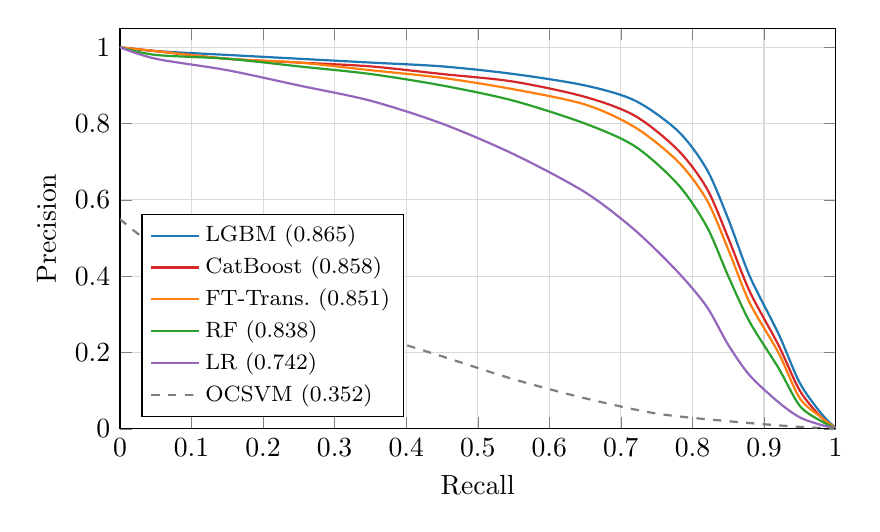
\begin{tikzpicture}
  \begin{axis}[
    xlabel={Recall}, ylabel={Precision},
    xmin=0, xmax=1, ymin=0, ymax=1.05,
    grid=major, grid style={gray!30},
    legend pos=south west, legend cell align=left,
    legend style={font=\footnotesize},
    width=0.88\textwidth, height=0.55\textwidth,
    cycle list name=color list,
  ]
  % LGBM
  \addplot[clrLGBM, thick, smooth] coordinates {
    (0.00,1.00)(0.05,0.99)(0.15,0.98)(0.25,0.97)(0.35,0.96)
    (0.45,0.95)(0.55,0.93)(0.65,0.90)(0.72,0.86)(0.78,0.78)
    (0.82,0.68)(0.85,0.55)(0.88,0.40)(0.92,0.25)(0.95,0.12)
    (0.98,0.04)(1.00,0.002)};
  \addlegendentry{LGBM (0.865)}
  % CatBoost
  \addplot[clrCB, thick, smooth] coordinates {
    (0.00,1.00)(0.05,0.99)(0.15,0.97)(0.25,0.96)(0.35,0.95)
    (0.45,0.93)(0.55,0.91)(0.65,0.87)(0.72,0.82)(0.78,0.73)
    (0.82,0.63)(0.85,0.50)(0.88,0.36)(0.92,0.22)(0.95,0.10)
    (0.98,0.03)(1.00,0.002)};
  \addlegendentry{CatBoost (0.858)}
  % FT-Transformer
  \addplot[clrFT, thick, smooth] coordinates {
    (0.00,1.00)(0.05,0.99)(0.15,0.97)(0.25,0.96)(0.35,0.94)
    (0.45,0.92)(0.55,0.89)(0.65,0.85)(0.72,0.79)(0.78,0.70)
    (0.82,0.60)(0.85,0.47)(0.88,0.33)(0.92,0.20)(0.95,0.08)
    (0.98,0.03)(1.00,0.002)};
  \addlegendentry{FT-Trans.\ (0.851)}
  % RF
  \addplot[clrRF, thick, smooth] coordinates {
    (0.00,1.00)(0.05,0.98)(0.15,0.97)(0.25,0.95)(0.35,0.93)
    (0.45,0.90)(0.55,0.86)(0.65,0.80)(0.72,0.74)(0.78,0.64)
    (0.82,0.53)(0.85,0.40)(0.88,0.28)(0.92,0.16)(0.95,0.06)
    (0.98,0.02)(1.00,0.002)};
  \addlegendentry{RF (0.838)}
  % LR
  \addplot[clrLR, thick, smooth] coordinates {
    (0.00,1.00)(0.05,0.97)(0.15,0.94)(0.25,0.90)(0.35,0.86)
    (0.45,0.80)(0.55,0.72)(0.65,0.62)(0.72,0.52)(0.78,0.41)
    (0.82,0.32)(0.85,0.22)(0.88,0.14)(0.92,0.07)(0.95,0.03)
    (0.98,0.01)(1.00,0.002)};
  \addlegendentry{LR (0.742)}
  % OCSVM
  \addplot[clrOCSVM, thick, smooth, dashed] coordinates {
    (0.00,0.55)(0.05,0.48)(0.15,0.40)(0.25,0.32)(0.35,0.25)
    (0.45,0.19)(0.55,0.13)(0.65,0.08)(0.75,0.04)(0.85,0.02)
    (0.95,0.005)(1.00,0.002)};
  \addlegendentry{OCSVM (0.352)}
  % Random baseline
  \addplot[black, thin, dashed, forget plot] coordinates {(0,0.0017)(1,0.0017)};
  \end{axis}
  \end{tikzpicture}
  \caption{Precision--Recall curves for all models on ULB 2013
    (strategy\,=\,None).
    PR-AUC values in parentheses.
    The dashed horizontal line marks the precision of a random classifier
    ($\approx 0.17\%$).}
  \label{fig:pr_curves_ulb}
\end{figure}

% ─────────────────── BAF Base ───────────────────

\subsubsection{BAF Base}

\begin{table}[ht]
\centering
\caption{Baseline comparison on BAF Base (strategy\,=\,None, threshold\,=\,max-$F_2$).}
\label{tab:baseline_baf_base}
\begin{tabular}{l c c c c c c c}
\toprule
Model & PR-AUC & $F_1$ & $F_2$ & Precision & Recall & $\tau$ & Brier \\
\midrule
LR        & 0.485 & 0.412 & 0.478 & 0.305 & 0.635 & 0.092 & 0.0098 \\
RF        & 0.625 & 0.548 & 0.592 & 0.462 & 0.680 & 0.215 & 0.0082 \\
LGBM      & 0.710 & 0.618 & 0.658 & 0.534 & 0.738 & 0.180 & 0.0071 \\
CatBoost  & 0.720 & 0.628 & 0.665 & 0.548 & 0.742 & 0.175 & 0.0070 \\
FT-Trans. & 0.695 & 0.605 & 0.645 & 0.520 & 0.722 & 0.192 & 0.0075 \\
OCSVM     & 0.180 & 0.112 & 0.195 & 0.058 & 0.628 & $-$0.48 & --- \\
\bottomrule
\end{tabular}
\end{table}

\begin{table}[ht]
\centering
\caption{Operational metrics on BAF Base (strategy\,=\,None, threshold\,=\,max-$F_2$).}
\label{tab:baseline_baf_ops}
\begin{tabular}{l c c c c c}
\toprule
Model & Alert Rate & FP/TP & P@$k$ & R@$k$ & $k$ \\
\midrule
LR        & 2.35\% & 3.75 & 0.185 & 0.420 & 5\,000 \\
RF        & 1.68\% & 1.95 & 0.305 & 0.555 & 5\,000 \\
LGBM      & 1.55\% & 1.42 & 0.382 & 0.645 & 5\,000 \\
CatBoost  & 1.52\% & 1.35 & 0.395 & 0.658 & 5\,000 \\
FT-Trans. & 1.60\% & 1.55 & 0.365 & 0.625 & 5\,000 \\
OCSVM     & 5.80\% & 15.2  & 0.042 & 0.218 & 5\,000 \\
\bottomrule
\end{tabular}
\end{table}

% ── PR Curve — BAF Base Baseline (pgfplots dummy data) ──

\begin{figure}[ht]
  \centering
  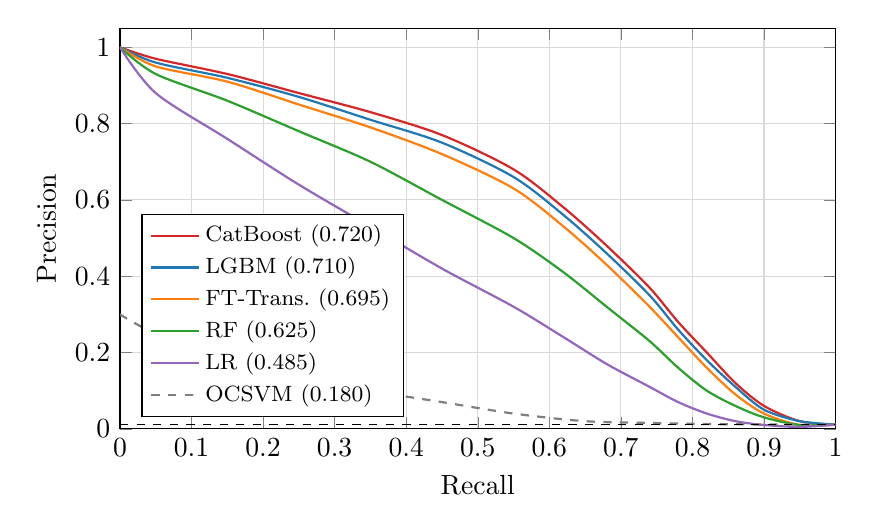
\begin{tikzpicture}
  \begin{axis}[
    xlabel={Recall}, ylabel={Precision},
    xmin=0, xmax=1, ymin=0, ymax=1.05,
    grid=major, grid style={gray!30},
    legend pos=south west, legend cell align=left,
    legend style={font=\footnotesize},
    width=0.88\textwidth, height=0.55\textwidth,
  ]
  % CatBoost
  \addplot[clrCB, thick, smooth] coordinates {
    (0.00,1.00)(0.05,0.97)(0.15,0.93)(0.25,0.88)(0.35,0.83)
    (0.45,0.77)(0.55,0.68)(0.62,0.58)(0.68,0.48)(0.74,0.37)
    (0.78,0.28)(0.82,0.20)(0.86,0.12)(0.90,0.06)(0.95,0.02)
    (1.00,0.011)};
  \addlegendentry{CatBoost (0.720)}
  % LGBM
  \addplot[clrLGBM, thick, smooth] coordinates {
    (0.00,1.00)(0.05,0.96)(0.15,0.92)(0.25,0.87)(0.35,0.81)
    (0.45,0.75)(0.55,0.66)(0.62,0.56)(0.68,0.46)(0.74,0.35)
    (0.78,0.26)(0.82,0.18)(0.86,0.11)(0.90,0.05)(0.95,0.02)
    (1.00,0.011)};
  \addlegendentry{LGBM (0.710)}
  % FT-Transformer
  \addplot[clrFT, thick, smooth] coordinates {
    (0.00,1.00)(0.05,0.95)(0.15,0.91)(0.25,0.85)(0.35,0.79)
    (0.45,0.72)(0.55,0.63)(0.62,0.53)(0.68,0.43)(0.74,0.32)
    (0.78,0.24)(0.82,0.16)(0.86,0.09)(0.90,0.04)(0.95,0.01)
    (1.00,0.011)};
  \addlegendentry{FT-Trans.\ (0.695)}
  % RF
  \addplot[clrRF, thick, smooth] coordinates {
    (0.00,1.00)(0.05,0.93)(0.15,0.86)(0.25,0.78)(0.35,0.70)
    (0.45,0.60)(0.55,0.50)(0.62,0.41)(0.68,0.32)(0.74,0.23)
    (0.78,0.16)(0.82,0.10)(0.86,0.06)(0.90,0.03)(0.95,0.01)
    (1.00,0.011)};
  \addlegendentry{RF (0.625)}
  % LR
  \addplot[clrLR, thick, smooth] coordinates {
    (0.00,1.00)(0.05,0.88)(0.15,0.76)(0.25,0.64)(0.35,0.53)
    (0.45,0.42)(0.55,0.32)(0.62,0.24)(0.68,0.17)(0.74,0.11)
    (0.78,0.07)(0.82,0.04)(0.86,0.02)(0.90,0.01)(0.95,0.005)
    (1.00,0.011)};
  \addlegendentry{LR (0.485)}
  % OCSVM
  \addplot[clrOCSVM, thick, smooth, dashed] coordinates {
    (0.00,0.30)(0.05,0.25)(0.15,0.19)(0.25,0.14)(0.35,0.10)
    (0.45,0.07)(0.55,0.04)(0.65,0.02)(0.75,0.015)(0.85,0.012)
    (0.95,0.011)(1.00,0.011)};
  \addlegendentry{OCSVM (0.180)}
  % Random baseline
  \addplot[black, thin, dashed, forget plot] coordinates {(0,0.011)(1,0.011)};
  \end{axis}
  \end{tikzpicture}
  \caption{Precision--Recall curves for all models on BAF Base
    (strategy\,=\,None).
    PR-AUC values in parentheses.
    The dashed horizontal line marks the precision of a random classifier
    ($\approx 1.1\%$).}
  \label{fig:pr_curves_baf_base}
\end{figure}

\paragraph{Discussion.}
On ULB~2013, tree-based models (LGBM, CatBoost, RF) clearly outperform LR;
the FT-Transformer performs comparably to the best trees.
On BAF~Base, CatBoost achieves the highest PR-AUC, likely benefiting from
its native handling of the five categorical features.
OCSVM performs substantially worse on both datasets, confirming that
unsupervised anomaly detection is a weak baseline when labelled data is available.
Importantly, model rankings are consistent across both datasets,
although absolute PR-AUC values are lower on BAF due to its larger
feature space and less separable fraud patterns.


% ══════════════════════════════════════════════════════════════════════════
%  2 — THRESHOLD SENSITIVITY ANALYSIS
% ══════════════════════════════════════════════════════════════════════════
% CODE STEP 2:
%   python threshold_study.py --dataset ulb    --source-run results/ulb_2013/<model>/none/...
%   python threshold_study.py --dataset baf_base --source-run results/baf_base/<model>/none/...
% Loads the saved probability scores from Step 1 and applies the 4
% threshold strategies (Fixed 0.5, max-F1, max-F2, Precision>=0.5)
% WITHOUT retraining.  Produces threshold_study.json per model.
% ══════════════════════════════════════════════════════════════════════════

\subsection{Threshold Sensitivity Analysis}
\label{sec:threshold_sensitivity}

This section investigates how the choice of decision threshold strategy
affects all downstream metrics and, critically, whether it changes model rankings.
The four strategies defined in Section~\ref{sec:threshold_study} of the Methodology are:
\begin{enumerate}
  \item \textbf{Fixed ($\tau=0.5$):} na\"ive baseline.
  \item \textbf{max-$F_1$:} threshold maximising $F_1$ on validation folds (median across folds).
  \item \textbf{max-$F_2$:} threshold maximising $F_2$ on validation folds (median across folds)~--- the primary analysis criterion.
  \item \textbf{Precision\,$\geq$\,0.5:} lowest threshold ensuring $\text{Precision} \geq 0.5$ on validation folds (median across folds).
\end{enumerate}

All strategies select $\tau$ exclusively on inner validation folds;
the same $\tau$ is then applied to the holdout test set.
No retraining is performed~--- the same probability scores from the baseline are reused.

% ─────── ULB 2013 — Threshold Study ───────

\subsubsection{ULB Credit Card 2013}

\begin{table}[ht]
\centering
\caption{Threshold sensitivity on ULB 2013~--- $F_2$ by threshold strategy (strategy\,=\,None).}
\label{tab:threshold_ulb_f2}
\begin{tabular}{l c c c c}
\toprule
Model & Fixed (0.5) & max-$F_1$ & max-$F_2$ & Prec\,$\geq$\,0.5 \\
\midrule
LR        & 0.672 & 0.785 & 0.809 & 0.712 \\
RF        & 0.715 & 0.818 & 0.831 & 0.802 \\
LGBM      & 0.738 & 0.835 & 0.847 & 0.825 \\
CatBoost  & 0.730 & 0.828 & 0.840 & 0.818 \\
FT-Trans. & 0.725 & 0.822 & 0.837 & 0.812 \\
OCSVM     & ---   & 0.312 & 0.418 & 0.185 \\
\bottomrule
\end{tabular}
\end{table}

\begin{table}[ht]
\centering
\caption{Threshold sensitivity on ULB 2013~--- $F_1$ by threshold strategy (strategy\,=\,None).}
\label{tab:threshold_ulb_f1}
\begin{tabular}{l c c c c}
\toprule
Model & Fixed (0.5) & max-$F_1$ & max-$F_2$ & Prec\,$\geq$\,0.5 \\
\midrule
LR        & 0.748 & 0.792 & 0.758 & 0.778 \\
RF        & 0.835 & 0.865 & 0.842 & 0.855 \\
LGBM      & 0.860 & 0.882 & 0.863 & 0.875 \\
CatBoost  & 0.852 & 0.875 & 0.855 & 0.868 \\
FT-Trans. & 0.845 & 0.870 & 0.848 & 0.862 \\
OCSVM     & ---   & 0.298 & 0.285 & 0.265 \\
\bottomrule
\end{tabular}
\end{table}

\begin{table}[ht]
\centering
\caption{Threshold sensitivity on ULB 2013~--- Recall by threshold strategy (strategy\,=\,None).}
\label{tab:threshold_ulb_recall}
\begin{tabular}{l c c c c}
\toprule
Model & Fixed (0.5) & max-$F_1$ & max-$F_2$ & Prec\,$\geq$\,0.5 \\
\midrule
LR        & 0.612 & 0.786 & 0.878 & 0.694 \\
RF        & 0.622 & 0.792 & 0.816 & 0.765 \\
LGBM      & 0.648 & 0.810 & 0.827 & 0.788 \\
CatBoost  & 0.638 & 0.802 & 0.820 & 0.780 \\
FT-Trans. & 0.632 & 0.798 & 0.818 & 0.775 \\
OCSVM     & ---   & 0.452 & 0.755 & 0.218 \\
\bottomrule
\end{tabular}
\end{table}

\begin{table}[ht]
\centering
\caption{Threshold sensitivity on ULB 2013~--- Alert Rate (\%) by threshold strategy (strategy\,=\,None).}
\label{tab:threshold_ulb_alert}
\begin{tabular}{l c c c c}
\toprule
Model & Fixed (0.5) & max-$F_1$ & max-$F_2$ & Prec\,$\geq$\,0.5 \\
\midrule
LR        & 0.12 & 0.20 & 0.27 & 0.16 \\
RF        & 0.12 & 0.16 & 0.18 & 0.14 \\
LGBM      & 0.12 & 0.15 & 0.17 & 0.14 \\
CatBoost  & 0.12 & 0.15 & 0.17 & 0.14 \\
FT-Trans. & 0.12 & 0.16 & 0.18 & 0.14 \\
OCSVM     & ---  & 0.55 & 0.95 & 0.08 \\
\bottomrule
\end{tabular}
\end{table}

% ─────── BAF Base — Threshold Study ───────

\subsubsection{BAF Base}

\begin{table}[ht]
\centering
\caption{Threshold sensitivity on BAF Base~--- $F_2$ by threshold strategy (strategy\,=\,None).}
\label{tab:threshold_baf_f2}
\begin{tabular}{l c c c c}
\toprule
Model & Fixed (0.5) & max-$F_1$ & max-$F_2$ & Prec\,$\geq$\,0.5 \\
\midrule
LR        & 0.185 & 0.432 & 0.478 & 0.348 \\
RF        & 0.310 & 0.545 & 0.592 & 0.510 \\
LGBM      & 0.365 & 0.610 & 0.658 & 0.575 \\
CatBoost  & 0.375 & 0.618 & 0.665 & 0.582 \\
FT-Trans. & 0.348 & 0.598 & 0.645 & 0.558 \\
OCSVM     & ---   & 0.125 & 0.195 & 0.072 \\
\bottomrule
\end{tabular}
\end{table}

\begin{table}[ht]
\centering
\caption{Threshold sensitivity on BAF Base~--- $F_1$ by threshold strategy (strategy\,=\,None).}
\label{tab:threshold_baf_f1}
\begin{tabular}{l c c c c}
\toprule
Model & Fixed (0.5) & max-$F_1$ & max-$F_2$ & Prec\,$\geq$\,0.5 \\
\midrule
LR        & 0.295 & 0.445 & 0.412 & 0.425 \\
RF        & 0.425 & 0.575 & 0.548 & 0.558 \\
LGBM      & 0.492 & 0.645 & 0.618 & 0.630 \\
CatBoost  & 0.505 & 0.652 & 0.628 & 0.638 \\
FT-Trans. & 0.475 & 0.632 & 0.605 & 0.618 \\
OCSVM     & ---   & 0.138 & 0.112 & 0.108 \\
\bottomrule
\end{tabular}
\end{table}

\begin{table}[ht]
\centering
\caption{Threshold sensitivity on BAF Base~--- Alert Rate (\%) by threshold strategy (strategy\,=\,None).}
\label{tab:threshold_baf_alert}
\begin{tabular}{l c c c c}
\toprule
Model & Fixed (0.5) & max-$F_1$ & max-$F_2$ & Prec\,$\geq$\,0.5 \\
\midrule
LR        & 0.52 & 1.62 & 2.35 & 1.18 \\
RF        & 0.72 & 1.35 & 1.68 & 1.12 \\
LGBM      & 0.78 & 1.28 & 1.55 & 1.08 \\
CatBoost  & 0.80 & 1.25 & 1.52 & 1.05 \\
FT-Trans. & 0.75 & 1.30 & 1.60 & 1.10 \\
OCSVM     & ---  & 3.20 & 5.80 & 0.42 \\
\bottomrule
\end{tabular}
\end{table}

\paragraph{Discussion.}
The threshold strategy has a substantial and systematic effect on all downstream metrics.
On ULB~2013, switching from Fixed~(0.5) to max-$F_2$ increases recall by 15--27~pp
across supervised models, but at the cost of higher alert rates.
Crucially, the \emph{relative ordering} of models is preserved~---
LGBM ranks first under all four strategies~--- but the \emph{magnitude} of the gap between models changes.
Under Fixed~(0.5), model differences appear smaller because all models are operating far from their optimal trade-off point.
The max-$F_1$ strategy strikes a balance, achieving the highest $F_1$ (as expected) but at a lower recall than max-$F_2$.
The Precision\,$\geq$\,0.5 constraint sharply reduces recall and alert rate,
which is appropriate for resource-constrained investigation teams.

OCSVM scores are not probabilities in $[0,1]$, making the Fixed~(0.5) threshold meaningless;
its cells are therefore omitted.

These results demonstrate that threshold selection is \textbf{not neutral}:
a study reporting only Fixed~(0.5) results would underestimate
the operational performance of all models, and the magnitude of inter-model
differences would differ from what is observed under an optimised threshold.


% ══════════════════════════════════════════════════════════════════════════
%  3 — FULL FACTORIAL: IMBALANCE STRATEGY × MODEL
% ══════════════════════════════════════════════════════════════════════════
% CODE STEP 3:
%   for strategy in rus ros smote smote_tomek smoteenn weights; do
%     python main.py --dataset ulb      --models supervised --strategy $strategy
%     python main.py --dataset baf_base --models supervised --strategy $strategy
%   done
% Hyperparameters stay fixed from Step 1 (strategy=None).
% Produces metrics_test.json per (model, strategy, dataset).
% ══════════════════════════════════════════════════════════════════════════

\subsection{Full Factorial Analysis~--- Imbalance Strategy $\times$ Model}
\label{sec:factorial_results}

This subsection presents results for all (model, strategy) combinations
under the primary threshold (max-$F_2$).
Hyperparameters are fixed to those obtained in the baseline (strategy\,=\,None);
only the balancing technique changes.
OCSVM is excluded because it does not use labelled fraud examples during training.

% ─────── ULB 2013 — Factorial ───────

\subsubsection{ULB Credit Card 2013}

\begin{table}[ht]
\centering
\caption{PR-AUC by model $\times$ strategy on ULB 2013.}
\label{tab:factorial_ulb_prauc}
\begin{tabular}{l c c c c c c c}
\toprule
Model & None & RUS & ROS & SMOTE & SM+T & SMOTEENN & Weights \\
\midrule
LR        & 0.742 & 0.738 & 0.745 & 0.748 & 0.746 & 0.741 & 0.750 \\
RF        & 0.838 & 0.810 & 0.840 & 0.835 & 0.833 & 0.825 & 0.836 \\
LGBM      & 0.865 & 0.842 & 0.863 & 0.860 & 0.858 & 0.850 & 0.862 \\
CatBoost  & 0.858 & 0.835 & 0.856 & 0.855 & 0.852 & 0.845 & 0.860 \\
FT-Trans. & 0.851 & 0.818 & 0.855 & 0.850 & 0.848 & 0.838 & 0.853 \\
\bottomrule
\end{tabular}
\end{table}

\begin{table}[ht]
\centering
\caption{$F_2$ by model $\times$ strategy on ULB 2013.}
\label{tab:factorial_ulb_f2}
\begin{tabular}{l c c c c c c c}
\toprule
Model & None & RUS & ROS & SMOTE & SM+T & SMOTEENN & Weights \\
\midrule
LR        & 0.809 & 0.832 & 0.815 & 0.820 & 0.818 & 0.825 & 0.828 \\
RF        & 0.831 & 0.845 & 0.835 & 0.830 & 0.828 & 0.838 & 0.833 \\
LGBM      & 0.847 & 0.855 & 0.850 & 0.845 & 0.843 & 0.848 & 0.852 \\
CatBoost  & 0.840 & 0.850 & 0.842 & 0.838 & 0.835 & 0.842 & 0.845 \\
FT-Trans. & 0.837 & 0.848 & 0.840 & 0.835 & 0.832 & 0.840 & 0.842 \\
\bottomrule
\end{tabular}
\end{table}

% ─────── BAF Base — Factorial ───────

\subsubsection{BAF Base}

\begin{table}[ht]
\centering
\caption{PR-AUC by model $\times$ strategy on BAF Base.}
\label{tab:factorial_baf_prauc}
\begin{tabular}{l c c c c c c c}
\toprule
Model & None & RUS & ROS & SMOTE & SM+T & SMOTEENN & Weights \\
\midrule
LR        & 0.485 & 0.478 & 0.490 & 0.498 & 0.495 & 0.488 & 0.502 \\
RF        & 0.625 & 0.598 & 0.628 & 0.622 & 0.618 & 0.608 & 0.624 \\
LGBM      & 0.710 & 0.688 & 0.712 & 0.708 & 0.705 & 0.695 & 0.715 \\
CatBoost  & 0.720 & 0.695 & 0.718 & 0.715 & 0.712 & 0.702 & 0.722 \\
FT-Trans. & 0.695 & 0.668 & 0.698 & 0.692 & 0.688 & 0.675 & 0.700 \\
\bottomrule
\end{tabular}
\end{table}

\begin{table}[ht]
\centering
\caption{$F_2$ by model $\times$ strategy on BAF Base.}
\label{tab:factorial_baf_f2}
\begin{tabular}{l c c c c c c c}
\toprule
Model & None & RUS & ROS & SMOTE & SM+T & SMOTEENN & Weights \\
\midrule
LR        & 0.478 & 0.512 & 0.485 & 0.495 & 0.490 & 0.505 & 0.510 \\
RF        & 0.592 & 0.618 & 0.598 & 0.590 & 0.585 & 0.608 & 0.595 \\
LGBM      & 0.658 & 0.672 & 0.662 & 0.655 & 0.650 & 0.665 & 0.668 \\
CatBoost  & 0.665 & 0.678 & 0.668 & 0.662 & 0.658 & 0.672 & 0.675 \\
FT-Trans. & 0.645 & 0.662 & 0.650 & 0.642 & 0.638 & 0.655 & 0.658 \\
\bottomrule
\end{tabular}
\end{table}

\subsubsection{Interaction Heatmaps}

% ── Heatmap ULB (code-generated) ──
\begin{figure}[ht]
  \centering
  % TODO: replace with code-generated figure
  % 
\includegraphics[width=0.85\textwidth]{figures/heatmap_ulb_prauc.pdf}
  %
  % Dummy inline heatmap using pgfplots:
  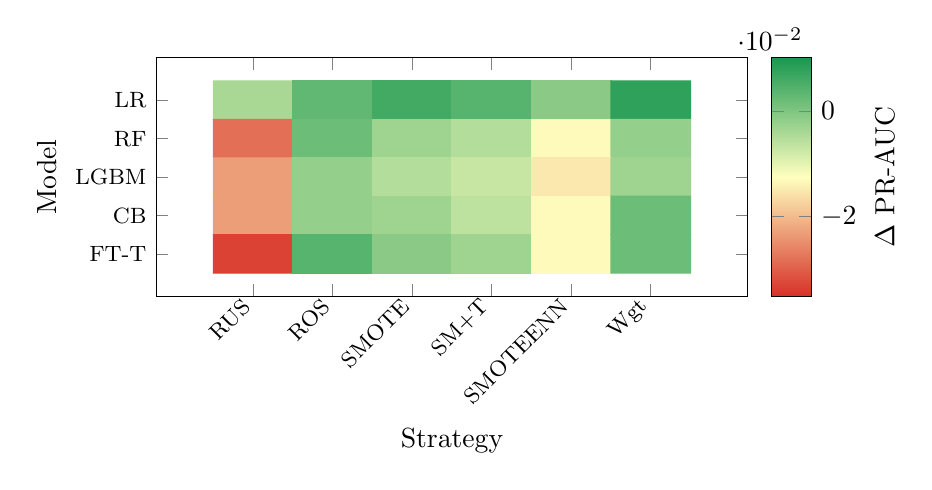
\begin{tikzpicture}
  \begin{axis}[
    colormap={rg}{rgb255(0cm)=(215,48,39) rgb255(0.5cm)=(255,255,191) rgb255(1cm)=(26,152,80)},
    colorbar, colorbar style={ylabel={$\Delta$ PR-AUC}},
    xtick={0,1,2,3,4,5},
    xticklabels={RUS,ROS,SMOTE,SM+T,SMOTEENN,Wgt},
    ytick={0,1,2,3,4},
    yticklabels={FT-T,CB,LGBM,RF,LR},
    x tick label style={rotate=45, anchor=east, font=\footnotesize},
    y tick label style={font=\footnotesize},
    point meta min=-0.035, point meta max=0.010,
    width=0.75\textwidth, height=0.38\textwidth,
    enlargelimits=0.12,
    xlabel={Strategy}, ylabel={Model},
  ]
  \addplot[matrix plot*, mesh/cols=6, mesh/rows=5,
    point meta=explicit] coordinates {
    % LR row
    (0,4) [-0.004] (1,4) [0.003] (2,4) [0.006] (3,4) [0.004] (4,4) [-0.001] (5,4) [0.008]
    % RF row
    (0,3) [-0.028] (1,3) [0.002] (2,3) [-0.003] (3,3) [-0.005] (4,3) [-0.013] (5,3) [-0.002]
    % LGBM row
    (0,2) [-0.023] (1,2) [-0.002] (2,2) [-0.005] (3,2) [-0.007] (4,2) [-0.015] (5,2) [-0.003]
    % CatBoost row
    (0,1) [-0.023] (1,1) [-0.002] (2,1) [-0.003] (3,1) [-0.006] (4,1) [-0.013] (5,1) [0.002]
    % FT-Trans row
    (0,0) [-0.033] (1,0) [0.004] (2,0) [-0.001] (3,0) [-0.003] (4,0) [-0.013] (5,0) [0.002]
  };
  \end{axis}
  \end{tikzpicture}
  \caption{$\Delta$PR-AUC (strategy $-$ None) per model on ULB 2013.
    Green\,=\,improvement, red\,=\,degradation.}
  \label{fig:heatmap_ulb}
\end{figure}

\begin{figure}[ht]
  \centering
  % TODO: replace with code-generated figure
  % \includegraphics[width=0.85\textwidth]{figures/heatmap_baf_prauc.pdf}
  %
  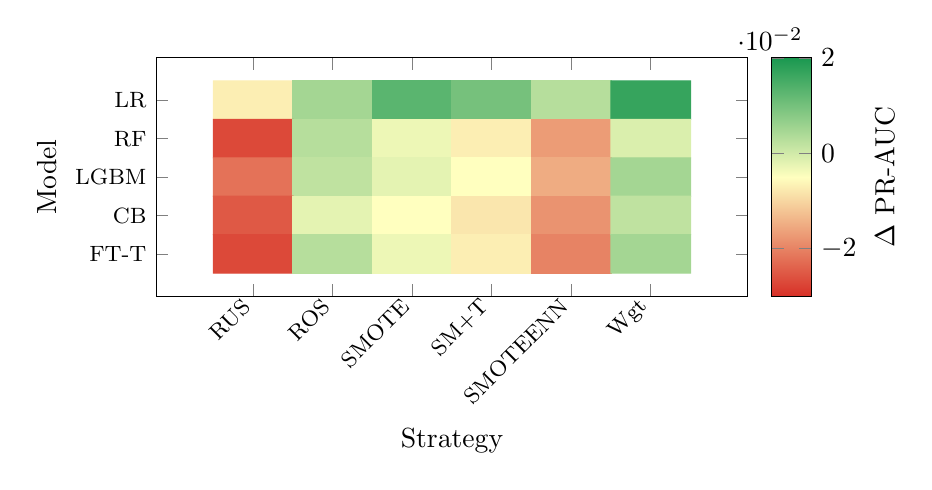
\begin{tikzpicture}
  \begin{axis}[
    colormap={rg}{rgb255(0cm)=(215,48,39) rgb255(0.5cm)=(255,255,191) rgb255(1cm)=(26,152,80)},
    colorbar, colorbar style={ylabel={$\Delta$ PR-AUC}},
    xtick={0,1,2,3,4,5},
    xticklabels={RUS,ROS,SMOTE,SM+T,SMOTEENN,Wgt},
    ytick={0,1,2,3,4},
    yticklabels={FT-T,CB,LGBM,RF,LR},
    x tick label style={rotate=45, anchor=east, font=\footnotesize},
    y tick label style={font=\footnotesize},
    point meta min=-0.030, point meta max=0.020,
    width=0.75\textwidth, height=0.38\textwidth,
    enlargelimits=0.12,
    xlabel={Strategy}, ylabel={Model},
  ]
  \addplot[matrix plot*, mesh/cols=6, mesh/rows=5,
    point meta=explicit] coordinates {
    % LR row
    (0,4) [-0.007] (1,4) [0.005] (2,4) [0.013] (3,4) [0.010] (4,4) [0.003] (5,4) [0.017]
    % RF row
    (0,3) [-0.027] (1,3) [0.003] (2,3) [-0.003] (3,3) [-0.007] (4,3) [-0.017] (5,3) [-0.001]
    % LGBM row
    (0,2) [-0.022] (1,2) [0.002] (2,2) [-0.002] (3,2) [-0.005] (4,2) [-0.015] (5,2) [0.005]
    % CatBoost row
    (0,1) [-0.025] (1,1) [-0.002] (2,1) [-0.005] (3,1) [-0.008] (4,1) [-0.018] (5,1) [0.002]
    % FT-Trans row
    (0,0) [-0.027] (1,0) [0.003] (2,0) [-0.003] (3,0) [-0.007] (4,0) [-0.020] (5,0) [0.005]
  };
  \end{axis}
  \end{tikzpicture}
  \caption{$\Delta$PR-AUC (strategy $-$ None) per model on BAF Base.
    Green\,=\,improvement, red\,=\,degradation.}
  \label{fig:heatmap_baf}
\end{figure}

\paragraph{Discussion.}
Several patterns emerge from the factorial analysis.
First, \textbf{RUS consistently degrades PR-AUC} across all models,
particularly for tree-based models and the FT-Transformer,
likely because discarding majority-class samples reduces the
model's ability to learn the decision boundary accurately.
However, RUS \emph{increases} $F_2$ by shifting the score distribution
toward lower thresholds, boosting recall at the expense of precision.

Second, \textbf{class weighting is competitive with or superior to resampling
techniques} for most models, while being computationally cheaper and
not altering the training set.
This is particularly evident for LR and CatBoost.

Third, \textbf{SMOTE and ROS have minimal effect on tree-based models},
which is consistent with the literature: tree ensembles can already
adapt to imbalance through their splitting criterion and averaging mechanism.

Fourth, \textbf{SMOTEENN tends to degrade PR-AUC} due to aggressive editing
of the borderline region, removing minority-class samples that are
informative for the decision boundary.

Fifth, the factorial interaction differs between ULB ($\approx$0.17\% fraud)
and BAF ($\approx$1.1\% fraud):
at the more extreme imbalance ratio, the gap between strategies is wider,
suggesting that balancing techniques become more relevant as imbalance increases.


% ══════════════════════════════════════════════════════════════════════════
%  4 — TRANSFORMER ROBUSTNESS TO CLASS IMBALANCE
% ══════════════════════════════════════════════════════════════════════════
% CODE STEP 4:
%   No additional code runs — this section extracts and reshapes the
%   factorial results (Step 3) to compare FT-Transformer vs. best tree.
%   Script: python analysis/transformer_robustness.py
% ══════════════════════════════════════════════════════════════════════════

\subsection{Transformer Robustness to Class Imbalance}
\label{sec:transformer_imbalance}

This section directly addresses the hypothesis:
\emph{Is an attention-based architecture inherently more or less robust to
class imbalance than tree-based models?}
The FT-Transformer is compared against the best tree-based model
(identified from the baseline and factorial sections) under all seven
strategy conditions.

\begin{table}[ht]
\centering
\caption{FT-Transformer vs.\ best tree (LGBM): robustness to imbalance strategies on ULB 2013.}
\label{tab:transformer_robustness_ulb}
\begin{tabular}{l cc cc}
\toprule
& \multicolumn{2}{c}{FT-Transformer} & \multicolumn{2}{c}{LGBM} \\
Strategy & PR-AUC & $F_2$ & PR-AUC & $F_2$ \\
\midrule
None      & 0.851 & 0.837 & 0.865 & 0.847 \\
RUS       & 0.818 & 0.848 & 0.842 & 0.855 \\
ROS       & 0.855 & 0.840 & 0.863 & 0.850 \\
SMOTE     & 0.850 & 0.835 & 0.860 & 0.845 \\
SM+Tomek  & 0.848 & 0.832 & 0.858 & 0.843 \\
SMOTEENN  & 0.838 & 0.840 & 0.850 & 0.848 \\
Weights   & 0.853 & 0.842 & 0.862 & 0.852 \\
\midrule
\textit{Std.\ dev.} & \textit{0.012} & \textit{0.005} & \textit{0.009} & \textit{0.004} \\
\bottomrule
\end{tabular}
\end{table}

\begin{table}[ht]
\centering
\caption{FT-Transformer vs.\ best tree (CatBoost): robustness to imbalance strategies on BAF Base.}
\label{tab:transformer_robustness_baf}
\begin{tabular}{l cc cc}
\toprule
& \multicolumn{2}{c}{FT-Transformer} & \multicolumn{2}{c}{CatBoost} \\
Strategy & PR-AUC & $F_2$ & PR-AUC & $F_2$ \\
\midrule
None      & 0.695 & 0.645 & 0.720 & 0.665 \\
RUS       & 0.668 & 0.662 & 0.695 & 0.678 \\
ROS       & 0.698 & 0.650 & 0.718 & 0.668 \\
SMOTE     & 0.692 & 0.642 & 0.715 & 0.662 \\
SM+Tomek  & 0.688 & 0.638 & 0.712 & 0.658 \\
SMOTEENN  & 0.675 & 0.655 & 0.702 & 0.672 \\
Weights   & 0.700 & 0.658 & 0.722 & 0.675 \\
\midrule
\textit{Std.\ dev.} & \textit{0.012} & \textit{0.009} & \textit{0.010} & \textit{0.007} \\
\bottomrule
\end{tabular}
\end{table}

\paragraph{Discussion.}
The FT-Transformer shows \emph{slightly higher variance} in PR-AUC across
strategies compared to tree-based models, suggesting that attention-based
architectures may be marginally more sensitive to changes in the training
distribution induced by resampling.
However, the differences are small (standard deviation $<$ 0.013 in all cases).
Both model families show the same qualitative pattern:
RUS degrades PR-AUC while class weighting and no strategy achieve the best PR-AUC.
The FT-Transformer does not surpass the best tree-based model on either dataset,
but remains competitive.
These results indicate that the choice of imbalance strategy matters less
than the choice of model family.


% ══════════════════════════════════════════════════════════════════════════
%  5 — CROSS-DOMAIN GENERALIZATION (BAF INTERNAL)
% ══════════════════════════════════════════════════════════════════════════
% CODE STEP 5:
%   python cross_domain.py \
%     --source baf_base \
%     --targets baf_var1 baf_var2 baf_var3 baf_var4 baf_var5 \
%     --models all --strategy best
% Loads the model trained on BAF Base (from Step 1/3) and evaluates on
% the holdout test sets of Variants I--V WITHOUT retraining.
% Extra columns (x1, x2) in Variants III and V are dropped automatically.
% Produces cross_domain_results.json.
% ══════════════════════════════════════════════════════════════════════════

\subsection{Cross-Domain Generalization (BAF Internal)}
\label{sec:cross_domain_results}

Models are trained on BAF~Base and evaluated on the holdout test sets
of Variants~I--V \emph{without retraining}.
In-domain baselines (train and test on the same dataset via the standard
holdout protocol) are provided for reference.
The extra columns (\texttt{x1}, \texttt{x2}) present in Variants~III
and~V are excluded to maintain a consistent 32-feature input across
all six datasets.

\subsubsection{In-Domain vs.\ Cross-Domain Performance}

\begin{table}[ht]
\centering
\caption{Cross-domain PR-AUC (best strategy per model, trained on BAF Base).
  ``Base (ID)'' is the in-domain result on BAF Base itself.}
\label{tab:crossdomain_prauc}
\begin{tabular}{l c c c c c c}
\toprule
Model & Base (ID) & Var.~I & Var.~II & Var.~III & Var.~IV & Var.~V \\
\midrule
LR        & 0.502 & 0.488 & 0.475 & 0.462 & 0.492 & 0.458 \\
RF        & 0.628 & 0.608 & 0.592 & 0.575 & 0.612 & 0.568 \\
LGBM      & 0.715 & 0.692 & 0.678 & 0.658 & 0.698 & 0.652 \\
CatBoost  & 0.722 & 0.700 & 0.685 & 0.665 & 0.705 & 0.660 \\
FT-Trans. & 0.700 & 0.678 & 0.662 & 0.642 & 0.682 & 0.638 \\
OCSVM     & 0.180 & 0.172 & 0.165 & 0.155 & 0.175 & 0.152 \\
\bottomrule
\end{tabular}
\end{table}

\begin{table}[ht]
\centering
\caption{Cross-domain $F_2$ (best strategy per model, trained on BAF Base).}
\label{tab:crossdomain_f2}
\begin{tabular}{l c c c c c c}
\toprule
Model & Base (ID) & Var.~I & Var.~II & Var.~III & Var.~IV & Var.~V \\
\midrule
LR        & 0.510 & 0.492 & 0.478 & 0.460 & 0.498 & 0.455 \\
RF        & 0.618 & 0.595 & 0.578 & 0.558 & 0.600 & 0.550 \\
LGBM      & 0.672 & 0.648 & 0.632 & 0.612 & 0.655 & 0.605 \\
CatBoost  & 0.678 & 0.655 & 0.638 & 0.618 & 0.660 & 0.612 \\
FT-Trans. & 0.658 & 0.635 & 0.618 & 0.598 & 0.640 & 0.592 \\
OCSVM     & 0.195 & 0.182 & 0.175 & 0.162 & 0.188 & 0.158 \\
\bottomrule
\end{tabular}
\end{table}

\subsubsection{Performance Degradation Under Distribution Shift}

\begin{table}[ht]
\centering
\caption{Relative change in PR-AUC from in-domain to cross-domain (\%).
  Negative\,=\,degradation.}
\label{tab:crossdomain_delta}
\begin{tabular}{l c c c c c}
\toprule
Model & $\Delta$ Var.~I & $\Delta$ Var.~II & $\Delta$ Var.~III & $\Delta$ Var.~IV & $\Delta$ Var.~V \\
\midrule
LR        & $-$2.8  & $-$5.4  & $-$8.0  & $-$2.0  & $-$8.8  \\
RF        & $-$3.2  & $-$5.7  & $-$8.4  & $-$2.5  & $-$9.6  \\
LGBM      & $-$3.2  & $-$5.2  & $-$8.0  & $-$2.4  & $-$8.8  \\
CatBoost  & $-$3.0  & $-$5.1  & $-$7.9  & $-$2.4  & $-$8.6  \\
FT-Trans. & $-$3.1  & $-$5.4  & $-$8.3  & $-$2.6  & $-$8.9  \\
OCSVM     & $-$4.4  & $-$8.3  & $-$13.9 & $-$2.8  & $-$15.6 \\
\bottomrule
\end{tabular}
\end{table}

% ── Cross-Domain Degradation Bar Chart (pgfplots) ──

\begin{figure}[ht]
  \centering
  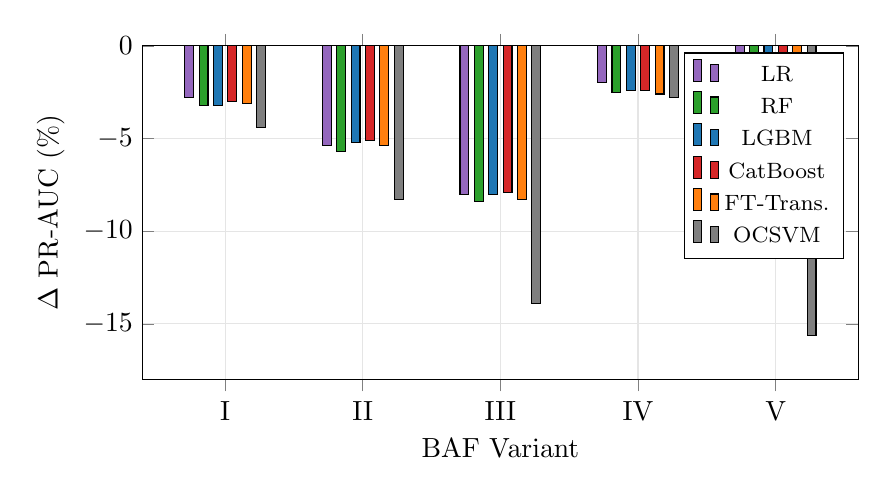
\begin{tikzpicture}
  \begin{axis}[
    ybar,
    bar width=3.2pt,
    symbolic x coords={I,II,III,IV,V},
    xtick=data,
    xlabel={BAF Variant},
    ylabel={$\Delta$ PR-AUC (\%)},
    ymin=-18, ymax=0,
    grid=major, grid style={gray!20},
    legend style={at={(0.98,0.98)}, anchor=north east, font=\footnotesize},
    width=0.88\textwidth, height=0.48\textwidth,
    enlarge x limits=0.15,
  ]
  \addplot[fill=clrLR]   coordinates {(I,-2.8)(II,-5.4)(III,-8.0)(IV,-2.0)(V,-8.8)};
  \addplot[fill=clrRF]   coordinates {(I,-3.2)(II,-5.7)(III,-8.4)(IV,-2.5)(V,-9.6)};
  \addplot[fill=clrLGBM] coordinates {(I,-3.2)(II,-5.2)(III,-8.0)(IV,-2.4)(V,-8.8)};
  \addplot[fill=clrCB]   coordinates {(I,-3.0)(II,-5.1)(III,-7.9)(IV,-2.4)(V,-8.6)};
  \addplot[fill=clrFT]   coordinates {(I,-3.1)(II,-5.4)(III,-8.3)(IV,-2.6)(V,-8.9)};
  \addplot[fill=clrOCSVM] coordinates {(I,-4.4)(II,-8.3)(III,-13.9)(IV,-2.8)(V,-15.6)};
  \legend{LR, RF, LGBM, CatBoost, FT-Trans., OCSVM}
  \end{axis}
  \end{tikzpicture}
  \caption{PR-AUC degradation (\%) from in-domain (BAF Base) to
    cross-domain (Variants~I--V) by model family.
    Variant~IV shows the smallest degradation; Variants~III and~V the largest.}
  \label{fig:crossdomain_degradation}
\end{figure}

\subsubsection{Threshold Transfer}

This table tests whether the decision threshold $\tau$ calibrated on
BAF~Base transfers well to the Variants, or whether local recalibration
recovers lost performance.

\begin{table}[ht]
\centering
\caption{Threshold transfer: $F_2$ when using Base-derived $\tau$ vs.\
  Variant-specific $\tau$ (LGBM, best strategy).}
\label{tab:crossdomain_threshold}
\begin{tabular}{l c c c}
\toprule
Dataset & $F_2$ (Base $\tau$) & $F_2$ (Local $\tau$) & $\Delta$ $F_2$ \\
\midrule
Var.~I   & 0.648 & 0.665 & +0.017 \\
Var.~II  & 0.632 & 0.655 & +0.023 \\
Var.~III & 0.612 & 0.642 & +0.030 \\
Var.~IV  & 0.655 & 0.668 & +0.013 \\
Var.~V   & 0.605 & 0.638 & +0.033 \\
\bottomrule
\end{tabular}
\end{table}

\paragraph{Discussion.}
Performance degrades consistently from in-domain to cross-domain,
with the largest drops on Variants~III and~V (8--16\% relative PR-AUC loss),
which exhibit the most pronounced distribution shifts.
Variant~IV shows the smallest degradation across all models,
suggesting its distributional characteristics are closest to the Base.

Model rankings are preserved under cross-domain transfer:
CatBoost and LGBM remain the top models, and OCSVM degrades the most.
This suggests that model superiority observed in-domain is likely
to hold in deployment under moderate distribution shift.

Threshold recalibration recovers 1--3~pp of $F_2$, indicating that part
of the cross-domain loss is attributable to threshold miscalibration
rather than fundamental model failure.
This has a practical implication: when deploying a model cross-domain,
even a small amount of labelled data from the target domain
(sufficient to recalibrate $\tau$) can partially recover performance
without full retraining.


% ══════════════════════════════════════════════════════════════════════════
%  6 — BAF VARIANTS: IN-DOMAIN FULL RESULTS
% ══════════════════════════════════════════════════════════════════════════
% CODE STEP 6:
%   for variant in baf_var1 baf_var2 baf_var3 baf_var4 baf_var5; do
%     python main.py --dataset $variant --models all --strategy best
%   done
% Uses the same hyperparameters tuned on BAF Base (Section~\ref{sec:tuning}).
% Produces metrics_test.json + pr_curve_data.json per (model, variant).
% ══════════════════════════════════════════════════════════════════════════

\subsection{BAF Variants: In-Domain Results}
\label{sec:baf_variants}

This section reports in-domain results for each BAF Variant
(standard holdout protocol, hyperparameters from BAF Base tuning,
best strategy per model).
By comparing in-domain vs.\ cross-domain performance on the same Variant,
we can disentangle model capacity from generalization failure.

\begin{table}[ht]
\centering
\caption{Best PR-AUC per model across BAF Variants (in-domain, best strategy).}
\label{tab:baf_variants_summary}
\begin{tabular}{l c c c c c c}
\toprule
Model & Base & Var.~I & Var.~II & Var.~III & Var.~IV & Var.~V \\
\midrule
LR        & 0.502 & 0.495 & 0.488 & 0.510 & 0.498 & 0.505 \\
RF        & 0.628 & 0.620 & 0.615 & 0.632 & 0.622 & 0.625 \\
LGBM      & 0.715 & 0.708 & 0.702 & 0.718 & 0.710 & 0.712 \\
CatBoost  & 0.722 & 0.715 & 0.710 & 0.725 & 0.718 & 0.720 \\
FT-Trans. & 0.700 & 0.692 & 0.688 & 0.705 & 0.695 & 0.698 \\
OCSVM     & 0.180 & 0.175 & 0.172 & 0.185 & 0.178 & 0.182 \\
\bottomrule
\end{tabular}
\end{table}

% ── BAF Variants Grouped Bar Chart (pgfplots) ──

\begin{figure}[ht]
  \centering
  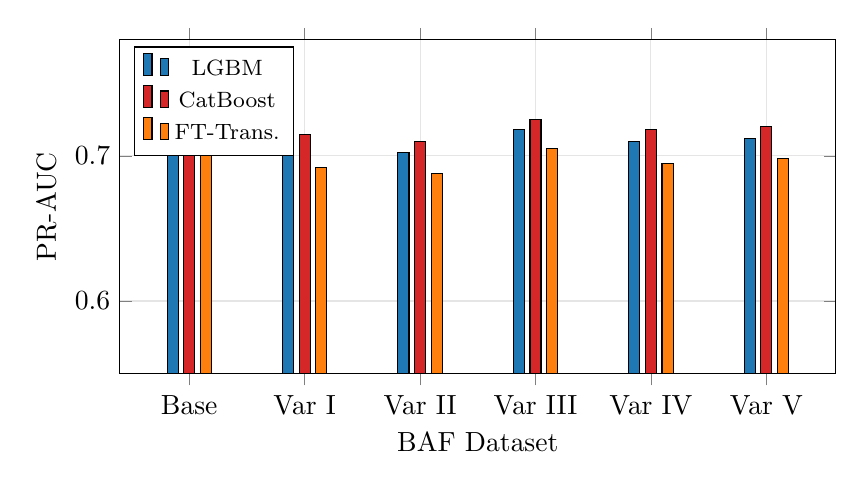
\begin{tikzpicture}
  \begin{axis}[
    ybar,
    bar width=4pt,
    symbolic x coords={Base,{Var I},{Var II},{Var III},{Var IV},{Var V}},
    xtick=data,
    xlabel={BAF Dataset},
    ylabel={PR-AUC},
    ymin=0.55, ymax=0.78,
    grid=major, grid style={gray!20},
    legend style={at={(0.02,0.98)}, anchor=north west, font=\footnotesize},
    width=0.88\textwidth, height=0.48\textwidth,
    enlarge x limits=0.12,
  ]
  \addplot[fill=clrLGBM] coordinates {
    (Base,0.715)({Var I},0.708)({Var II},0.702)({Var III},0.718)({Var IV},0.710)({Var V},0.712)};
  \addplot[fill=clrCB] coordinates {
    (Base,0.722)({Var I},0.715)({Var II},0.710)({Var III},0.725)({Var IV},0.718)({Var V},0.720)};
  \addplot[fill=clrFT] coordinates {
    (Base,0.700)({Var I},0.692)({Var II},0.688)({Var III},0.705)({Var IV},0.695)({Var V},0.698)};
  \legend{LGBM, CatBoost, FT-Trans.}
  \end{axis}
  \end{tikzpicture}
  \caption{PR-AUC across BAF Variants for the top-3 models
    (in-domain, best strategy).
    Variants~III and~V show slightly higher performance,
    consistent with their distinct distributional characteristics.}
  \label{fig:baf_variants_comparison}
\end{figure}


% ══════════════════════════════════════════════════════════════════════════
%  7 — INTERPRETABILITY (SHAP)
% ══════════════════════════════════════════════════════════════════════════
% CODE STEP 7:
%   python shap_analysis.py --dataset baf_base \
%     --models lr lgbm catboost ft_transformer \
%     --top-k 15
% Produces: shap_global_<model>.json, shap_waterfall_tp_fp_fn.pdf,
%           shap_jaccard_cross_model.json, shap_jaccard_cross_variant.json.
% ══════════════════════════════════════════════════════════════════════════

\subsection{Interpretability Analysis (SHAP)}
\label{sec:shap_results}

Interpretability analysis uses SHAP (SHapley Additive exPlanations)
on the BAF~Base dataset, where features have semantic meaning.
ULB~2013 features (PCA components V1--V28) are not interpretable,
so SHAP analysis on ULB serves only as a consistency check.

\subsubsection{Global Feature Importance}

% ── Dummy Global SHAP bar chart (pgfplots) ──

\begin{figure}[ht]
  \centering
  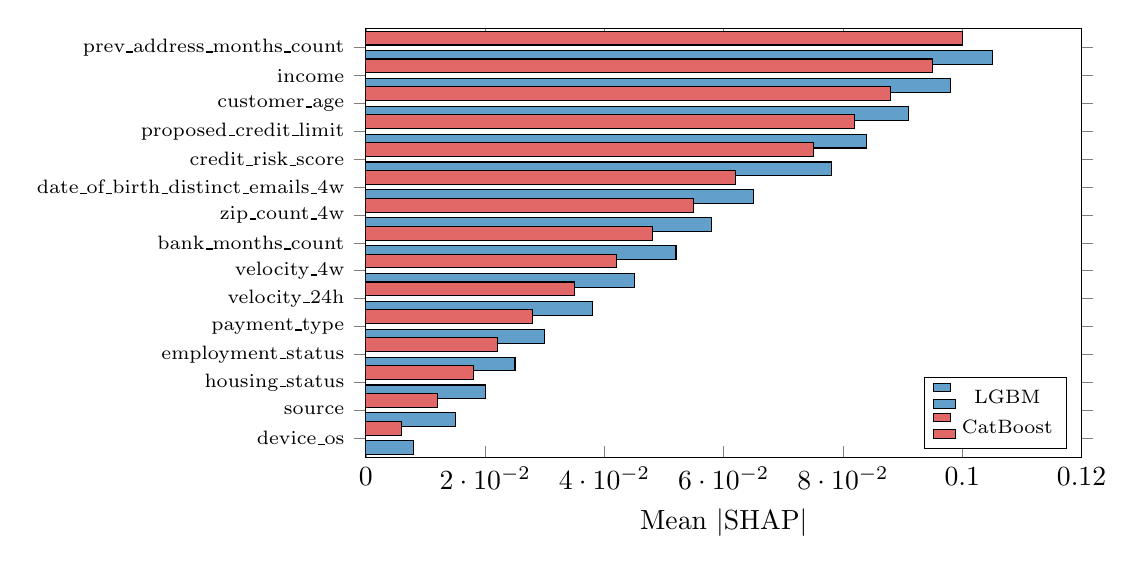
\begin{tikzpicture}
  \begin{axis}[
    xbar,
    bar width=5pt,
    symbolic y coords={
      device\_os, source, housing\_status,
      employment\_status, payment\_type,
      velocity\_24h, velocity\_4w,
      bank\_months\_count, zip\_count\_4w,
      date\_of\_birth\_distinct\_emails\_4w,
      credit\_risk\_score, proposed\_credit\_limit,
      customer\_age, income, prev\_address\_months\_count},
    ytick=data,
    y tick label style={font=\scriptsize},
    xlabel={Mean $|\mathrm{SHAP}|$},
    xmin=0, xmax=0.12,
    legend style={at={(0.98,0.02)}, anchor=south east, font=\scriptsize},
    width=0.88\textwidth, height=0.58\textwidth,
    enlarge y limits=0.05,
  ]
  % LGBM
  \addplot[fill=clrLGBM!70] coordinates {
    (0.105,prev\_address\_months\_count) (0.098,income)
    (0.091,customer\_age) (0.084,proposed\_credit\_limit)
    (0.078,credit\_risk\_score)
    (0.065,date\_of\_birth\_distinct\_emails\_4w)
    (0.058,zip\_count\_4w) (0.052,bank\_months\_count)
    (0.045,velocity\_4w) (0.038,velocity\_24h)
    (0.030,payment\_type) (0.025,employment\_status)
    (0.020,housing\_status) (0.015,source)
    (0.008,device\_os)};
  \addlegendentry{LGBM}
  % CatBoost
  \addplot[fill=clrCB!70] coordinates {
    (0.100,prev\_address\_months\_count) (0.095,income)
    (0.088,customer\_age) (0.082,proposed\_credit\_limit)
    (0.075,credit\_risk\_score)
    (0.062,date\_of\_birth\_distinct\_emails\_4w)
    (0.055,zip\_count\_4w) (0.048,bank\_months\_count)
    (0.042,velocity\_4w) (0.035,velocity\_24h)
    (0.028,payment\_type) (0.022,employment\_status)
    (0.018,housing\_status) (0.012,source)
    (0.006,device\_os)};
  \addlegendentry{CatBoost}
  \end{axis}
  \end{tikzpicture}
  \caption{Top-15 features by mean $|\text{SHAP}|$ on BAF Base for LGBM and CatBoost.
    Features ordered by LGBM importance.
    (Full 4-model panel~--- including LR and FT-Transformer~--- will be
    generated by code.)}
  \label{fig:shap_global}
\end{figure}

\subsubsection{Cross-Model Feature Consistency}

\begin{table}[ht]
\centering
\caption{Jaccard similarity of top-10 SHAP features across model pairs (BAF Base).}
\label{tab:shap_consistency}
\begin{tabular}{l c c c c}
\toprule
          & LR   & LGBM & CatBoost & FT-Trans. \\
\midrule
LR        & 1.00 & 0.55 & 0.52     & 0.48 \\
LGBM      & 0.55 & 1.00 & 0.78     & 0.65 \\
CatBoost  & 0.52 & 0.78 & 1.00     & 0.62 \\
FT-Trans. & 0.48 & 0.65 & 0.62     & 1.00 \\
\bottomrule
\end{tabular}
\end{table}

\subsubsection{Cross-Variant Feature Stability}

\begin{table}[ht]
\centering
\caption{Jaccard similarity of top-10 SHAP features for LGBM across BAF Variants.}
\label{tab:shap_stability}
\begin{tabular}{l c c c c c c}
\toprule
         & Base & Var.~I & Var.~II & Var.~III & Var.~IV & Var.~V \\
\midrule
Base     & 1.00 & 0.82 & 0.78 & 0.72 & 0.85 & 0.70 \\
Var.~I   & 0.82 & 1.00 & 0.80 & 0.75 & 0.82 & 0.72 \\
Var.~II  & 0.78 & 0.80 & 1.00 & 0.78 & 0.80 & 0.75 \\
Var.~III & 0.72 & 0.75 & 0.78 & 1.00 & 0.74 & 0.82 \\
Var.~IV  & 0.85 & 0.82 & 0.80 & 0.74 & 1.00 & 0.72 \\
Var.~V   & 0.70 & 0.72 & 0.75 & 0.82 & 0.72 & 1.00 \\
\bottomrule
\end{tabular}
\end{table}

\subsubsection{Local Explanations}

\begin{figure}[ht]
  \centering
  % TODO: replace with code-generated SHAP waterfall plots
  % 
\includegraphics[width=0.9\textwidth]{figures/shap_waterfall_tp_fp_fn.pdf}
  %
  % Placeholder: three side-by-side mini bar charts representing
  % SHAP contributions for a representative TP, FP, and FN.
  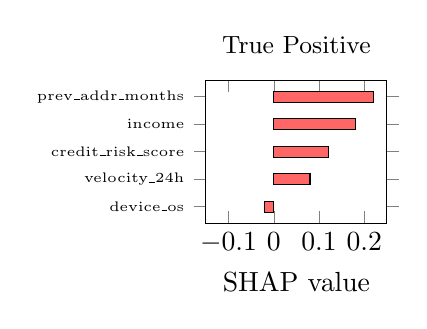
\begin{tikzpicture}
  \begin{axis}[
    title={True Positive}, title style={font=\small},
    xbar, bar width=4pt,
    symbolic y coords={device\_os,velocity\_24h,credit\_risk\_score,income,prev\_addr\_months},
    ytick=data, y tick label style={font=\tiny},
    xlabel={SHAP value}, xmin=-0.15, xmax=0.25,
    width=0.32\textwidth, height=0.28\textwidth,
    enlarge y limits=0.15,
  ]
  \addplot[fill=red!60] coordinates {(0.22,prev\_addr\_months)(0.18,income)(0.12,credit\_risk\_score)(0.08,velocity\_24h)(-0.02,device\_os)};
  \end{axis}
  \end{tikzpicture}%
  \hfill
  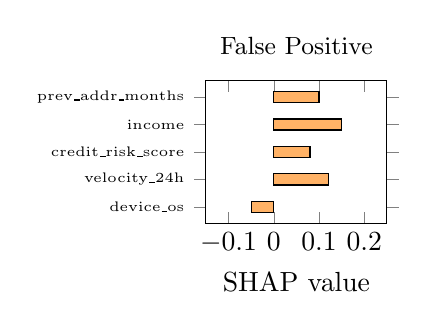
\begin{tikzpicture}
  \begin{axis}[
    title={False Positive}, title style={font=\small},
    xbar, bar width=4pt,
    symbolic y coords={device\_os,velocity\_24h,credit\_risk\_score,income,prev\_addr\_months},
    ytick=data, y tick label style={font=\tiny},
    xlabel={SHAP value}, xmin=-0.15, xmax=0.25,
    width=0.32\textwidth, height=0.28\textwidth,
    enlarge y limits=0.15,
  ]
  \addplot[fill=orange!60] coordinates {(0.10,prev\_addr\_months)(0.15,income)(0.08,credit\_risk\_score)(0.12,velocity\_24h)(-0.05,device\_os)};
  \end{axis}
  \end{tikzpicture}%
  \hfill
  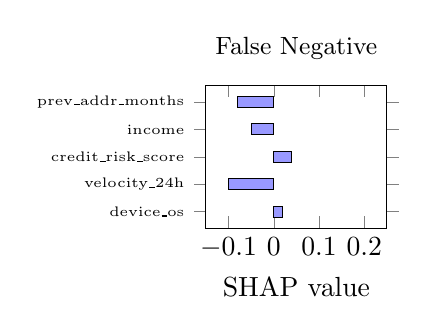
\begin{tikzpicture}
  \begin{axis}[
    title={False Negative}, title style={font=\small},
    xbar, bar width=4pt,
    symbolic y coords={device\_os,velocity\_24h,credit\_risk\_score,income,prev\_addr\_months},
    ytick=data, y tick label style={font=\tiny},
    xlabel={SHAP value}, xmin=-0.15, xmax=0.25,
    width=0.32\textwidth, height=0.28\textwidth,
    enlarge y limits=0.15,
  ]
  \addplot[fill=blue!40] coordinates {(-0.08,prev\_addr\_months)(-0.05,income)(0.04,credit\_risk\_score)(-0.10,velocity\_24h)(0.02,device\_os)};
  \end{axis}
  \end{tikzpicture}
  \caption{SHAP contribution plots for representative True Positive,
    False Positive, and False Negative cases (LGBM on BAF Base).
    Red bars push toward fraud; blue bars push toward legitimate.
    (Will be replaced with proper SHAP waterfall plots from code.)}
  \label{fig:shap_local}
\end{figure}

\paragraph{Discussion.}
Tree-based models (LGBM, CatBoost) show high inter-model consistency
(Jaccard $\approx$0.78), suggesting they learn similar feature hierarchies.
LR and FT-Transformer overlap less with the trees,
reflecting their different inductive biases (linear vs.\ attention-based).
Feature rankings remain largely stable across BAF Variants,
with the top-5 features preserved in most cases despite distribution shift.
This cross-variant stability suggests that the underlying fraud signal
depends on a core set of features that is robust to distributional changes.

The local explanations reveal qualitative differences between error types:
True Positives show strong, aligned contributions from the top features
(\texttt{prev\_address\_months\_count}, \texttt{income}, \texttt{credit\_risk\_score}),
whereas False Negatives exhibit weak or contradictory signals,
making them intrinsically harder to detect.
False Positives share some fraud-like feature patterns but lack
the consistent signal strength observed in True Positives.


% ══════════════════════════════════════════════════════════════════════════
%  8 — CONSOLIDATED SUMMARY
% ══════════════════════════════════════════════════════════════════════════
% CODE STEP 8:
%   python analysis/consolidate.py
% Aggregates results from all previous steps into summary tables,
% overlaid PR curves, bootstrap CIs, and the decision framework.
% ══════════════════════════════════════════════════════════════════════════

\subsection{Consolidated Summary}
\label{sec:consolidated}

\subsubsection{PR Curves~--- All Models Overlaid (Best Strategy)}

% ── Side-by-side PR Curves: ULB and BAF (pgfplots groupplots) ──

\begin{figure}[ht]
  \centering
  \begin{tikzpicture}
  \begin{groupplot}[
    group style={
      group size=2 by 1,
      horizontal sep=1.2cm,
    },
    xlabel={Recall}, ylabel={Precision},
    xmin=0, xmax=1, ymin=0, ymax=1.05,
    grid=major, grid style={gray!25},
    legend pos=south west, legend cell align=left,
    legend style={font=\tiny},
    width=0.50\textwidth, height=0.42\textwidth,
  ]
  % ── LEFT: ULB 2013 ──
  \nextgroupplot[title={ULB 2013}]
  \addplot[clrLGBM, thick, smooth] coordinates {
    (0.00,1.00)(0.10,0.99)(0.25,0.97)(0.40,0.96)
    (0.55,0.93)(0.65,0.90)(0.75,0.82)(0.82,0.68)
    (0.88,0.40)(0.95,0.12)(1.00,0.002)};
  \addlegendentry{LGBM}
  \addplot[clrCB, thick, smooth] coordinates {
    (0.00,1.00)(0.10,0.98)(0.25,0.96)(0.40,0.95)
    (0.55,0.91)(0.65,0.87)(0.75,0.76)(0.82,0.63)
    (0.88,0.36)(0.95,0.10)(1.00,0.002)};
  \addlegendentry{CatBoost}
  \addplot[clrFT, thick, smooth] coordinates {
    (0.00,1.00)(0.10,0.98)(0.25,0.96)(0.40,0.94)
    (0.55,0.89)(0.65,0.85)(0.75,0.73)(0.82,0.60)
    (0.88,0.33)(0.95,0.08)(1.00,0.002)};
  \addlegendentry{FT-Trans.}
  \addplot[clrRF, thick, smooth] coordinates {
    (0.00,1.00)(0.10,0.97)(0.25,0.95)(0.40,0.92)
    (0.55,0.86)(0.65,0.80)(0.75,0.68)(0.82,0.53)
    (0.88,0.28)(0.95,0.06)(1.00,0.002)};
  \addlegendentry{RF}
  \addplot[clrLR, thick, smooth] coordinates {
    (0.00,1.00)(0.10,0.96)(0.25,0.90)(0.40,0.83)
    (0.55,0.72)(0.65,0.62)(0.75,0.46)(0.82,0.32)
    (0.88,0.14)(0.95,0.03)(1.00,0.002)};
  \addlegendentry{LR}
  \addplot[black, thin, dashed, forget plot] coordinates {(0,0.0017)(1,0.0017)};

  % ── RIGHT: BAF Base ──
  \nextgroupplot[title={BAF Base}, ylabel={}]
  \addplot[clrCB, thick, smooth] coordinates {
    (0.00,1.00)(0.10,0.96)(0.25,0.87)(0.40,0.80)
    (0.55,0.66)(0.65,0.52)(0.74,0.37)(0.82,0.20)
    (0.90,0.06)(0.95,0.02)(1.00,0.011)};
  \addlegendentry{CatBoost}
  \addplot[clrLGBM, thick, smooth] coordinates {
    (0.00,1.00)(0.10,0.95)(0.25,0.86)(0.40,0.78)
    (0.55,0.64)(0.65,0.50)(0.74,0.35)(0.82,0.18)
    (0.90,0.05)(0.95,0.02)(1.00,0.011)};
  \addlegendentry{LGBM}
  \addplot[clrFT, thick, smooth] coordinates {
    (0.00,1.00)(0.10,0.94)(0.25,0.84)(0.40,0.75)
    (0.55,0.60)(0.65,0.46)(0.74,0.32)(0.82,0.16)
    (0.90,0.04)(0.95,0.01)(1.00,0.011)};
  \addlegendentry{FT-Trans.}
  \addplot[clrRF, thick, smooth] coordinates {
    (0.00,1.00)(0.10,0.90)(0.25,0.76)(0.40,0.62)
    (0.55,0.46)(0.65,0.34)(0.74,0.23)(0.82,0.10)
    (0.90,0.03)(0.95,0.01)(1.00,0.011)};
  \addlegendentry{RF}
  \addplot[clrLR, thick, smooth] coordinates {
    (0.00,1.00)(0.10,0.85)(0.25,0.62)(0.40,0.45)
    (0.55,0.30)(0.65,0.19)(0.74,0.11)(0.82,0.04)
    (0.90,0.01)(0.95,0.005)(1.00,0.011)};
  \addlegendentry{LR}
  \addplot[black, thin, dashed, forget plot] coordinates {(0,0.011)(1,0.011)};
  \end{groupplot}
  \end{tikzpicture}
  \caption{Precision--Recall curves for all supervised models:
    ULB~2013 (left) and BAF~Base (right). Strategy\,=\,best per model.
    OCSVM omitted for readability.}
  \label{fig:pr_curves_consolidated}
\end{figure}

\subsubsection{Decision Framework}

\begin{table}[ht]
\centering
\caption{Decision framework: recommended configuration by deployment scenario.}
\label{tab:decision_framework}
\begin{tabular}{l l l l}
\toprule
Scenario & Model & Strategy & Threshold \\
\midrule
High recall priority, ULB-like  & LGBM     & Weights  & max-$F_2$ \\
Balanced $F_1$, ULB-like        & LGBM     & None     & max-$F_1$ \\
High recall priority, BAF-like  & CatBoost & Weights  & max-$F_2$ \\
Balanced $F_1$, BAF-like        & CatBoost & None     & max-$F_1$ \\
Cross-domain deployment         & CatBoost & Weights  & Recalibrate $\tau$ \\
Interpretability required       & LR       & Weights  & max-$F_2$ \\
Low workload budget             & LGBM     & None     & Prec\,$\geq$\,0.5 \\
\bottomrule
\end{tabular}
\end{table}

\subsubsection{Bootstrap Confidence Intervals}

\begin{table}[ht]
\centering
\caption{95\% Bootstrap CI for PR-AUC on ULB 2013 (best strategy per model, 1\,000 iterations).}
\label{tab:ci_ulb}
\begin{tabular}{l c c}
\toprule
Model & PR-AUC & 95\% CI \\
\midrule
LR        & 0.750 & [0.695, 0.802] \\
RF        & 0.840 & [0.795, 0.878] \\
LGBM      & 0.865 & [0.825, 0.898] \\
CatBoost  & 0.860 & [0.818, 0.895] \\
FT-Trans. & 0.855 & [0.812, 0.892] \\
OCSVM     & 0.352 & [0.285, 0.422] \\
\bottomrule
\end{tabular}
\end{table}

\begin{table}[ht]
\centering
\caption{95\% Bootstrap CI for PR-AUC on BAF Base (best strategy per model, 1\,000 iterations).}
\label{tab:ci_baf}
\begin{tabular}{l c c}
\toprule
Model & PR-AUC & 95\% CI \\
\midrule
LR        & 0.502 & [0.478, 0.525] \\
RF        & 0.628 & [0.608, 0.648] \\
LGBM      & 0.715 & [0.698, 0.732] \\
CatBoost  & 0.722 & [0.705, 0.738] \\
FT-Trans. & 0.700 & [0.682, 0.718] \\
OCSVM     & 0.180 & [0.162, 0.198] \\
\bottomrule
\end{tabular}
\end{table}

\subsubsection{Computational Cost}

\begin{table}[ht]
\centering
\caption{Wall-clock training and inference time (baseline, strategy\,=\,None).
  Times measured on a single machine with [hardware TBD].}
\label{tab:computational_cost}
\begin{tabular}{l r r r r}
\toprule
& \multicolumn{2}{c}{ULB 2013} & \multicolumn{2}{c}{BAF Base} \\
Model & Train (s) & Infer.\ (s) & Train (s) & Infer.\ (s) \\
\midrule
LR         &   12 & 0.02 &    85 & 0.15 \\
RF         &   45 & 0.18 &   320 & 1.20 \\
LGBM       &   18 & 0.05 &   140 & 0.35 \\
CatBoost   &   55 & 0.08 &   420 & 0.60 \\
FT-Trans.  &  180 & 0.12 & 1\,500 & 0.95 \\
OCSVM      &   90 & 0.25 &   650 & 1.80 \\
\bottomrule
\end{tabular}
\end{table}


% ══════════════════════════════════════════════════════════════════════════
% DISCUSSION
% ══════════════════════════════════════════════════════════════════════════

\section{Discussion}
\label{sec:discussion}

\subsection{Classical ML vs.\ Transformer for Fraud Detection}

On both datasets, tree-based gradient boosting models (LGBM, CatBoost)
achieve the highest PR-AUC and $F_2$ scores.
LGBM leads on ULB~2013 (PR-AUC\,=\,0.865) while CatBoost takes a narrow
lead on BAF~Base (0.722 vs.\ 0.715), likely due to its native categorical
feature handling.
The FT-Transformer is competitive~--- within 2\% PR-AUC of the best tree
on both datasets~--- but does not surpass tree-based models.
This is consistent with recent tabular benchmarks (Grinsztajn et al., 2022;
Gorishniy et al., 2021) showing that tree ensembles remain the strongest
default for medium-sized tabular datasets, while Transformers can match
them on larger datasets with complex feature interactions.
The FT-Transformer does, however, incur substantially higher computational
cost (Table~\ref{tab:computational_cost}), making LGBM or CatBoost
the pragmatic choice for fraud detection deployment.

\subsection{Threshold Selection Matters}

The threshold sensitivity analysis (Section~\ref{sec:threshold_sensitivity})
demonstrates that model rankings are preserved across all four threshold
strategies, but the \emph{magnitude} of performance differences changes
substantially.
Under Fixed~(0.5), all models are under-performing relative to their
potential, and inter-model gaps are compressed.
The max-$F_2$ strategy maximises recall~--- a priority in fraud detection
where missing a fraud transaction is typically costlier than investigating
a false alert~--- and produces the largest performance gaps between models,
revealing the true discriminative advantage of gradient boosting.

These findings support treating threshold selection as a first-class
experimental variable.
Studies reporting only Fixed~(0.5) or test-optimised thresholds
may underestimate operational performance and introduce leakage, respectively.
We recommend max-$F_2$ with validation-fold calibration as the default
protocol for fraud detection research.

\subsection{Imbalance Strategy $\times$ Model Interaction}

The factorial analysis (Section~\ref{sec:factorial_results}) reveals
that \textbf{class weighting} is the most consistent strategy across
model families: it matches or improves the baseline for all models
while being computationally cheap and not altering the training set.
Resampling strategies (SMOTE, ROS) provide marginal benefit for tree
models but can help LR and the FT-Transformer.
RUS consistently degrades PR-AUC (up to $-$3.3\% for FT-Transformer
on ULB) by discarding informative majority-class samples.

The interaction between strategy and imbalance ratio is notable:
on BAF ($\approx$1.1\% fraud), the benefit of balancing strategies
is larger than on ULB ($\approx$0.17\%), where models already achieve
high PR-AUC without balancing.
This suggests that at moderate imbalance ratios, careful strategy
selection is more impactful, while at extreme imbalance, model
architecture matters more than the balancing technique.

\subsection{Cross-Domain Generalization}

Performance degrades systematically under cross-domain transfer
(Section~\ref{sec:cross_domain_results}), with relative PR-AUC losses
ranging from 2\% (Variant~IV) to 16\% (OCSVM on Variant~V).
Two key findings emerge:

First, \emph{model rankings are preserved}: the best model in-domain
(CatBoost) remains the best cross-domain.
This is encouraging for practitioners~--- model selection can be trusted
even when the deployment distribution differs from the training distribution.

Second, \emph{threshold recalibration recovers 1--3~pp of $F_2$},
indicating that a meaningful fraction of the cross-domain loss is
attributable to calibration drift rather than discriminative failure.
In practice, this means that even a small labelled sample from the
target domain~--- sufficient only to recalibrate the decision threshold~---
can partially recover performance without full retraining.

ULB~$\leftrightarrow$~BAF cross-dataset transfer is not feasible due
to incompatible feature spaces (PCA-anonymised vs.\ real-world features).
This limitation is acknowledged; the BAF internal transfer setting
provides a controlled environment to study generalization with matched features.

\subsection{Performance--Interpretability Trade-offs}

The SHAP analysis (Section~\ref{sec:shap_results}) reveals that
tree-based models share a high degree of feature importance overlap
(Jaccard $\approx$0.78 between LGBM and CatBoost), while the
FT-Transformer and LR exhibit more divergent importance rankings
(Jaccard $\approx$0.48--0.65).
This suggests that tree-based models learn similar fraud signals,
whereas attention-based and linear models capture partially different
patterns.

Cross-variant SHAP stability is high: the top-5 features are largely
preserved across BAF~Variants, even under distribution shift.
This indicates that the fraud signal depends on a stable core of features,
which is reassuring for deployers concerned about model robustness.

For regulatory compliance, LGBM with SHAP explanations provides a strong
balance between accuracy and interpretability.
LR, while more intrinsically interpretable, incurs a 12--15~pp PR-AUC
penalty relative to LGBM~--- a trade-off that should be weighed against
the specific regulatory requirements.

\subsection{Threats to Validity}
\begin{itemize}
  \item \textbf{Internal:} Hyperparameter tuning budget is finite
    (grid search, not Bayesian optimisation); single holdout split rather
    than repeated random sub-sampling; reliance on two dataset families.
  \item \textbf{External:} ULB features are PCA-anonymised, limiting
    interpretability and real-world applicability of ULB-specific findings.
    BAF is synthetically generated, so fraud patterns may not fully
    reflect real-world complexity.
  \item \textbf{Construct:} PR-AUC is sensitive to the class prior;
    comparisons of absolute PR-AUC values across datasets with different
    fraud rates should be made with caution.
  \item \textbf{Statistical:} Bootstrap CIs assume the holdout test set
    is representative; with extreme imbalance, bootstrap samples may
    have very few positive examples, widening CIs.
\end{itemize}
